\title{Architectural Views}
\maketitle

\section{Introduction}

Understanding software is hard.
It is often claimed that reading code is harder than writing code\footnote{Though evidence suggests that an ability to read and reason 
about code is necessary to learn how to program well \cite{lister-tracing-explaining-writing} \cite{lister-neo-piagetian}.}.
This principle is used to explain a programmers' innate desire to constantly rewrite their code from scratch.
If software is hard to understand, then software architecture is near impossible.
Fortunately, architects have developed a number of techniques to manage this complexity.

A software architecture consists of many dimensions.
Programming languages, communication protocols, the operating systems and hardware used, virtualisation used,
and the code itself are a subset of the many dimensions which comprise a software architecture.
Asking a programmer's monkey brain to understand, communicate, or document every dimension at once is needlessly cruel.
This is where architectural views come in.

Architectural views, or architectural projections, are a representation of one or more related aspects of a software architecture.
Views allow us to focus on a particular slice of our multi-dimensional software architecture, ignoring other irrelevant slices.
For example, if we are interested in applying a security patch to our software then we are only interested in the view
which tells us which software packages are used on each host machine.

The successful implementation of any architecture relies on the ability for the architectural views
to be disseminated, understood, and implemented.
For some organisations, the software is simple enough, or the team small enough, that the design
can be communicated through word of mouth.
As software becomes increasingly complex and developers number in the thousands,
it is critical for design to be communicated as effectively as possible.
In addition to facilitating communication,
architectural views also enable architectural policies to be designed and implemented.

The seminal architecture book, Software Architecture in Practice \cite{bass2021software},
categorises architectural views into three groups.
These three groups each answer different questions about the architecture, specifically:
\begin{description}
    \item[Module Views] How implementation components of a system are structured and depended upon.
    \item[Component-and-connector Views] How individual components communicate with each other.
    \item[Allocation Views] How the components are deployed to hardware.
\end{description}

\section{Module Views}
Module views are composed of modules, which are static units of functionality such as classes, functions, packages, or whole programs.
The defining characteristic of a module is that it represents software responsible for some well-defined functionality.
For example, a class which converts JSON to XML would be considered a module, as would a function which performs the same task.

The primary function of module views are to communicate the dependencies of a module.
Rarely does software work completely in isolation, often is it constructed with implicit or explicit dependencies.
A module which converts JSON to XML might depend upon a module which parses JSON and a module which can format XML.
Module views make these dependencies explicit.

\begin{figure}[ht]
\centering
\begin{subfigure}[b]{\textwidth}
\begin{shaded}
\begin{lstlisting}[style=python]
import json
import xml

class JSONtoXML:
    def load(self, json_file):
        with open(json_file) as f:
            data = json.load(f)
        self.data = self.convert(data)

    def export(self, xml_file):
        xml.write(xml_file, data)

    def convert(self, data: JSON) -> XML:
        ...
\end{lstlisting}
\end{shaded}
\caption{Pseudo-code to convert JSON to XML}
\end{subfigure}


\begin{subfigure}[b]{\textwidth}
\begin{center}
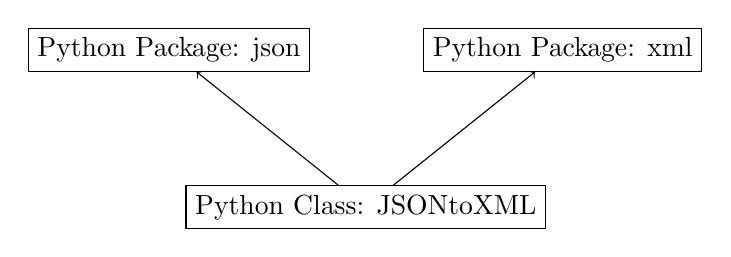
\begin{tikzpicture}
    \node[draw] (json) at (0,0) {Python Package: json};
    \node[draw] (xml) at (5,0) {Python Package: xml};
    \node[draw] (jsontoxml) at (2.5,-2) {Python Class: JSONtoXML};

    \path [->] (jsontoxml) edge node {} (json);
    \path [->] (jsontoxml) edge node {} (xml);
\end{tikzpicture}
\end{center}
\caption{An example of a module view which illustrates the dependencies of the \texttt{JSONtoXML} class}
\end{subfigure}
\caption{A simple module view of a JSON to XML program.}
\end{figure}

\section{Component-and-Connector Views}
Component-and-connector views focus on the runtime, or dynamic behaviour of a system.
Components are units which perform some computation or operation at runtime.
These components could overlap with the modules of a module view but are often at a higher level of abstraction.
The focus of component-and-connector views is how these components communicate at runtime.
Runtime communication is the connector of components.
For example, a service which registers users to a website might have new registrations communicated via a \link{REST}{https://www.ibm.com/cloud/learn/rest-apis} request.
The service may then communicate the new user information to a database via SQL queries.

When we look at software architecture, component-and-connector views are the most commonly used views.
They are common because they contain runtime information which is not easily automatically extracted.
Module views can be generated after the fact, i.e. it is easy enough for a project to generate a UML inheritance diagram.
Component-and-connector views are often something that is maintained manually by architects and developers.

\section{Allocation Views}
According to Bass et al, allocation views map the software's structures to the system's non-software structures \cite{bass2021software}.
They include the concepts of who is building which software elements,
where are source files stored for different activites such as development and testing,
and where are software elements executed.
The first two points are important for project management and build management.
The last point of how the software is executed on different processing nodes is important for architectural design.
This is sometimes called the \emph{deployment structure} or the software system's \emph{physical architecture}.

Understanding the physical architecture (simplistically the hardware\footnote{Whether it is virtualised or physical hardware}
on which the software is executed) is important when designing the software's \emph{logical architecture}.
Component-and-connector views describe the software's logical architecture.
This design of the logical architecture must contain components that can be allocated appropriately to processing nodes,
and these nodes must have communication links that enable the components to interact.

\section{On-line Store Example}
Consider a simple on-line store. It sells a number of different products. Customers can use both web and mobile applications providing to shop at the store.

\subsection{Allocation View}
Figure \ref{fig:deploymentDiagram} is an example allocation view of the system.
It is a UML deployment diagram showing the system's physical architecture
and some of the components that are deployed onto that structure.

\begin{figure}[h]
    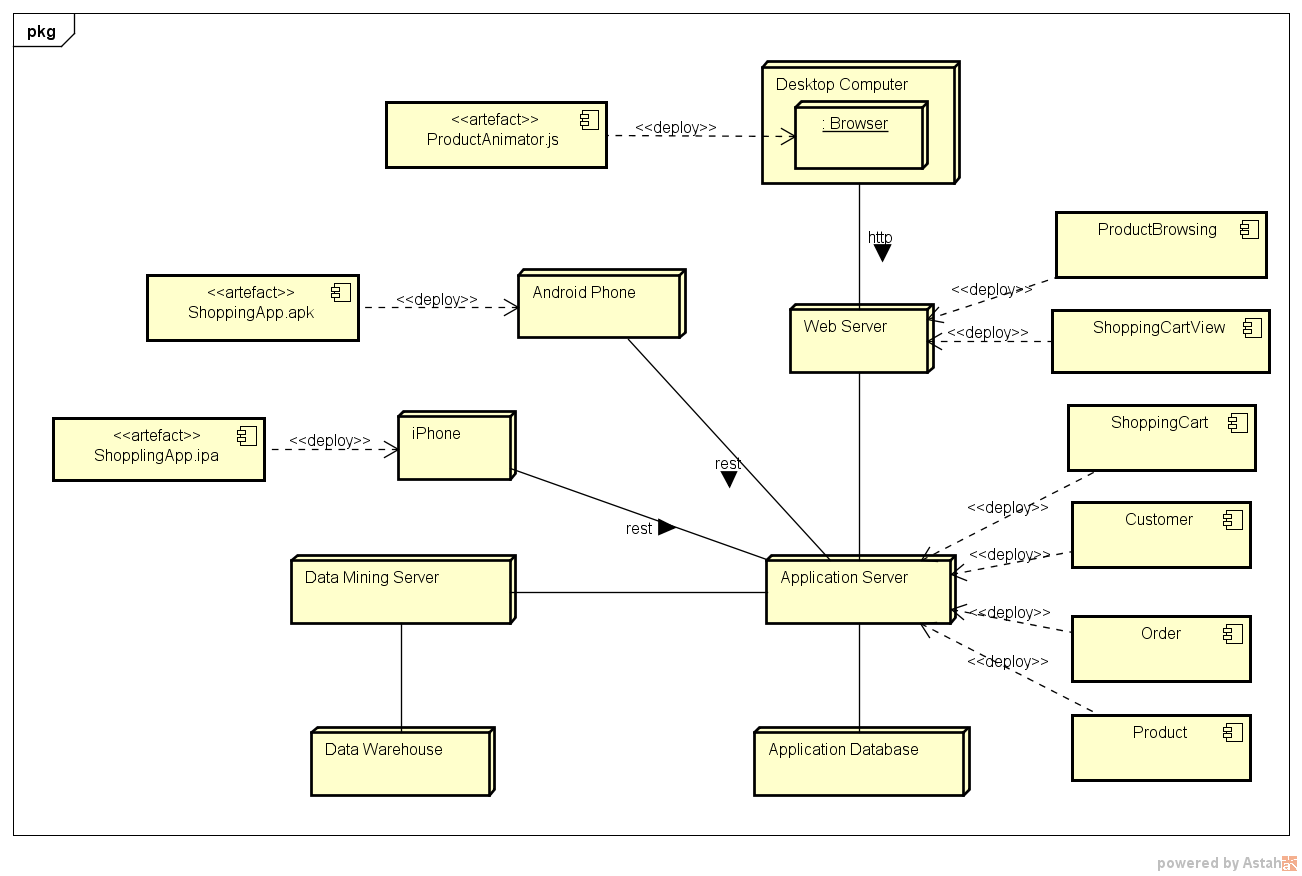
\includegraphics[trim=37 57 20 40,clip,width=\textwidth]{images/deployment_diagram.png}
    \caption{Example allocation view for an on-line store.}
    \label{fig:deploymentDiagram}
\end{figure}

There are both web and mobile applications that allow customers to shop at the store.
A web server handles browser requests from customers, using the HTTP protocol.
A JavaScript module called ProductAnimator is downloaded to the customer's browser to allow them to see interactive 3d views of products.
The ProductBrowsing and ShoppingCartView components run on the web server, providing those aspects of the user interaction.
The web server has a network connection to an application server, which provides the core logic of the on-line store.
Examples of components that would run on the application server are Customer, ShoppingCart, Order and Product.
The application server has network connections to a server running the application database and to a data mining server.
The data mining server has a network connection to a server running the data warehouse.
The mobile applications run on their respective phone environments and use REST API calls over the internet to interact with application server.

\subsection{Component-and-Connector View}
Figure \ref{fig:componentDiagram} is an example component-and-connector view of a small part of the system.
It is a UML component diagram showing the logical architecture of the components that allow customers to browse for products and add them to their shopping cart.

\begin{figure}[h]
    \centering
    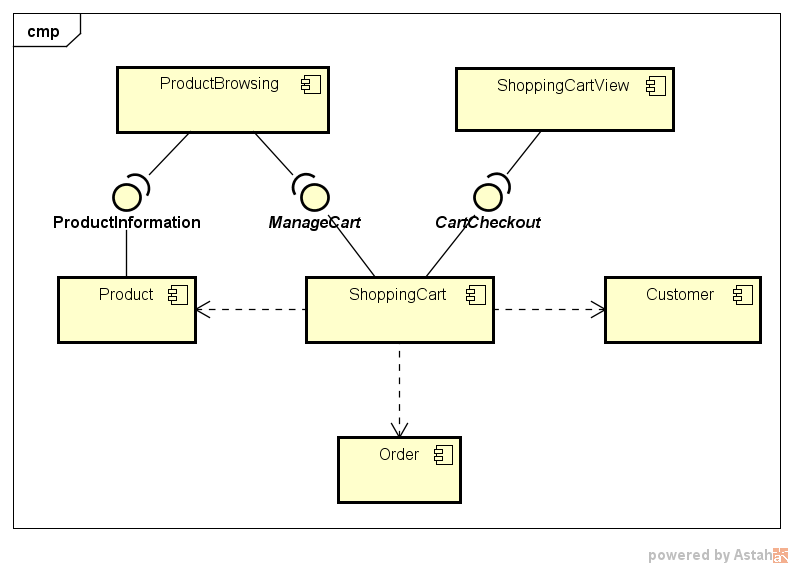
\includegraphics[trim=37 45 20 48,clip,width=0.75\textwidth]{images/component_diagram.png}
    \caption{Example component-and-connector view for part of an on-line store.}
    \label{fig:componentDiagram}
\end{figure}

As was shown in figure \ref{fig:deploymentDiagram}, the ProductBrowsing and ShoppingCartView components are deployed on the web server.
These two component provide the user interaction behaviour of browing for products, adding them to the shopping cart, and purchasing the products.
The Product, ShoppingCart, Order and Customer components are deployed on the application server.
These components deliver the logical behaviour of providing information about products, tracking what is in the shopping cart, and placing orders.
The ProductBrowsing component uses the ProductInformation and ManageCart interfaces.
These two interfaces are realised (or implemented) by the Product and ShoppingCart components respectively.
The ShoppingCartView component uses the CartCheckout interface, which is realised by the ShoppingCart component.
These interfaces describe the communication pathways between the components on the different nodes of the physical architecture.
The ShoppingCart component uses the Product, Customer and Order components.
At the programming level, there are likely to be interfaces between these components which are not shown in this diagram.

\subsection{Module View}
